\chapter{Latex-Grundbeispiele}\label{sec:neues_kapitel}

\section{Standards}
\glqq Anführungszeichen \grqq{}                          %Anführungszeichen unten:oben 
\grqq Anführungszeichen \grqq{}                          %Anführungszeichen oben:oben

\textbf{Fett gedruckt}                                   %Fett gedruckt

\begin{align}                                   % Formel
    F_{LO} = I*l*B \qquad | \qquad \vec{l}  \perp \vec{B} \label{formel:lorentz}
\end{align}

\subsection{Formeln direkt im Text}
$F_{LO} = I*l*B \qquad | \qquad \vec{l}\perp \vec{B}$            % auch Formel      

\subsection{Link}
\href{https://www.dsl-ltd.co.uk/what-are-single-board-computers-and-how-are-they-used/}{Link}


\subsection{Akronyme}
\acp{SBC}
\acf{SBC}
\subsection*{geschütztes Leerzeichen}
% Um ein geschütztes Leerzeichen bei einem Namen einzufügen, fügen Sie einfach eine Tilde (~) statt dem 
% Leerzeichen ein: B. ~Brecht. Beachten Sie in dem Fall, dass vor und nach der Tilde kein Leerzeichen 
% stehen darf.
5~V

\section{Aufzählungen}

\begin{itemize}                                         % nicht nummerierte Aufzählung
        \item $MINIFS(max_range, criteria_range1, criteria1, [criteria_range2, criteria2], ...)$
        \item $AVERAGEIFS(max_range, criteria_range1, criteria1, [criteria_range2, criteria2], ...)$
        \item $MAXIFS(max_range, criteria_range1, criteria1, [criteria_range2, criteria2], ...)$\cite{SBCs,fritzing}
\end{itemize}

\autoref{sec:neues_kapitel}                     % referenz auf abschnitt

\section{Listing}
\begin{lstlisting}[language=bash,caption={Installation und starten von Mosquitto auf dem Raspberry Pi},label={lst:inst_mosq}]
    sudo apt install mosquitto mosquitto-clients
    sudo systemctl start mosquitto

    sudo systemctl enable mosquitto
\end{lstlisting}

\chapter{Graphiken}

\section{Bild}
\begin{figure}[H]                               % Bild
    \center
    
\includegraphics[width=0.3\linewidth]{dhbw-logo.png}
    \caption{ABB Logo} \cite[58]{SBCs}
    \label{fig:abb_logo}
\end{figure}

\section{Zwei Bilder}
\begin{figure}[H]                                   %2 Bilder
    \centering
    \begin{subfigure}[b]{0.44\textwidth}
        \centering
        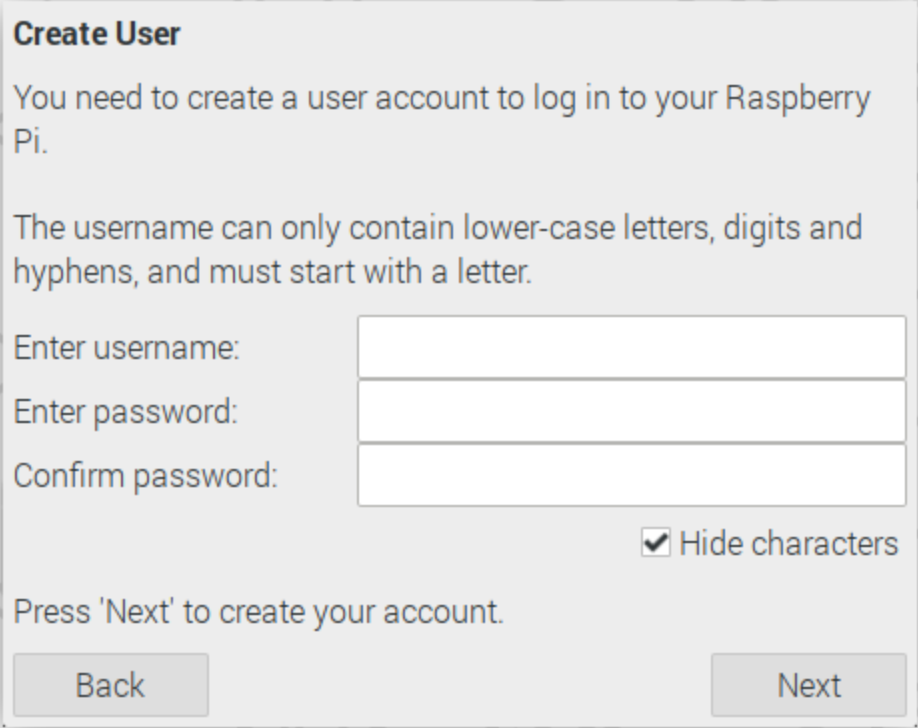
\includegraphics[width=\textwidth]{setup_rasp_user.png}
        \caption{Konfiguration des Benutzers auf dem Raspberry Pi} 
        \label{fig:setup_rasp_user}
    \end{subfigure}
    \hfill
    \begin{subfigure}[b]{0.44\textwidth}
        \centering
        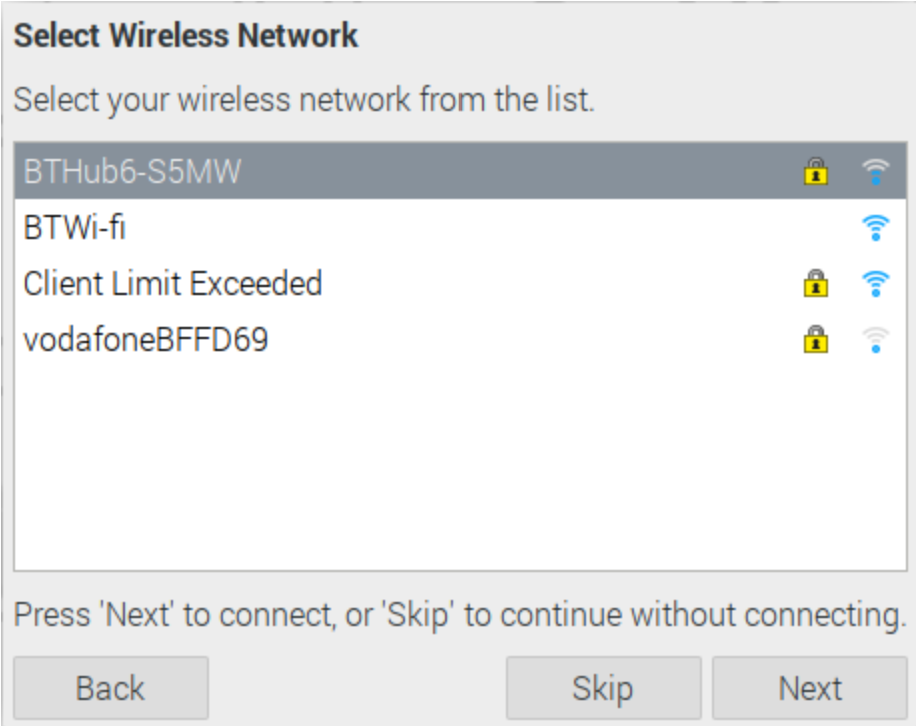
\includegraphics[width=\textwidth]{setup_rasp_wifi.png}
        \caption{Konfiguration der Netzwerkverbindung auf dem Raspberry Pi}
        \label{fig:setup_rasp_wifi}
    \end{subfigure}
    \caption*{\cite{ultraschallsensor_p&f}}
\end{figure}


\section{Tabellen}
\begin{table}                                   %einfache Tabelle
    \centering
    \caption{Klemmenbezeichnung}
    \begin{tabular}{|l|l|} \hline
        \textbf{Phase}                         & \textbf{Ux, Vx oder Wx}               \\ \hline
        Wicklungsanfang                        & x = 1                                 \\ \hline
        Wicklungsende                          & x = 2                                 \\ \hline                              
    \end{tabular}
    \caption*{\cite{SBCs}}
\end{table}

\begin{table}[H]                                                            %Tabelle mit mergen
    \centering
    \caption{Exemplarischer Auszug aus der Excel-Tabelle}
    \begin{tabular}{|c|c|c|c|c|} \hline
        \textbf{Anwendung/Motor}        & \textbf{Wert}     & \textbf{Motorleisung}         & \textbf{Erfolgsquote}     & \textbf{Preis}    \\ \hline
        \multirow{3}{*}{Schmelzepumpe}  & Min               & $575 \,kW$                    & \multirow{3}{*}{$14\%$}   & 100\euro      \\ \cline{2-3}\cline{5-5}
                                        & Average           & $1.680 \,kW$                  &                           & 200\euro      \\ \cline{2-3}\cline{5-5}
                                        & Max               & $3.500 \,kW$                  &                           & 200\euro      \\ \hline                 
        \multirow{3}{*}{AMI 450}        & Min               & $1.000 \,kW$                  & \multirow{3}{*}{$28\%$}   & 200 \euro      \\ \cline{2-3}\cline{5-5}
                                        & Average           & $1.328 \,kW$                  &                           & 200\euro      \\ \cline{2-3}\cline{5-5}
                                        & Max               & $1.750 \,kW$                  &                           & 200\euro      \\ \hline         
        \multirow{3}{*}{ACS1000}        & Min               & $435 \,kW$                    & \multirow{3}{*}{$29\%$}   & 200 \euro      \\ \cline{2-3}\cline{5-5}
                                        & Average           & $1.903 \,kW$                  &                           & 200\euro      \\ \cline{2-3}\cline{5-5}
                                        & Max               & $3.900 \,kW$                  &                           & 200\euro      \\ \hline 
    \end{tabular}
    \caption*{}
    \label{tab:test}
\end{table}


\section{Baumstrucktur}
\begin{figure}[H]
    \centering
    \begin{forest}
        forked edges,
        for tree={
            draw,
            align=center,
            edge={-latex},
            parent anchor=south,
            child anchor=north,
            calign=center,
            anchor=center,
            minimum width=2.3cm,
        }
        [smarthome
            [kueche]
            [wohnzimmer
                [rollo
                    [status]
                    [steuerung]
                    [modus]
                ]
                [messung
                    [licht]
                    [feuchtigkeit]
                    [temp]
                ]
            ]
            [badezimmer]
        ]
    \end{forest}
    \caption{Struktur der Topics in dem MQTT System}\label{fig:struk_topic}
\end{figure}

\section{Tikz Abbildung}
\begin{figure}[H]
    \centering
    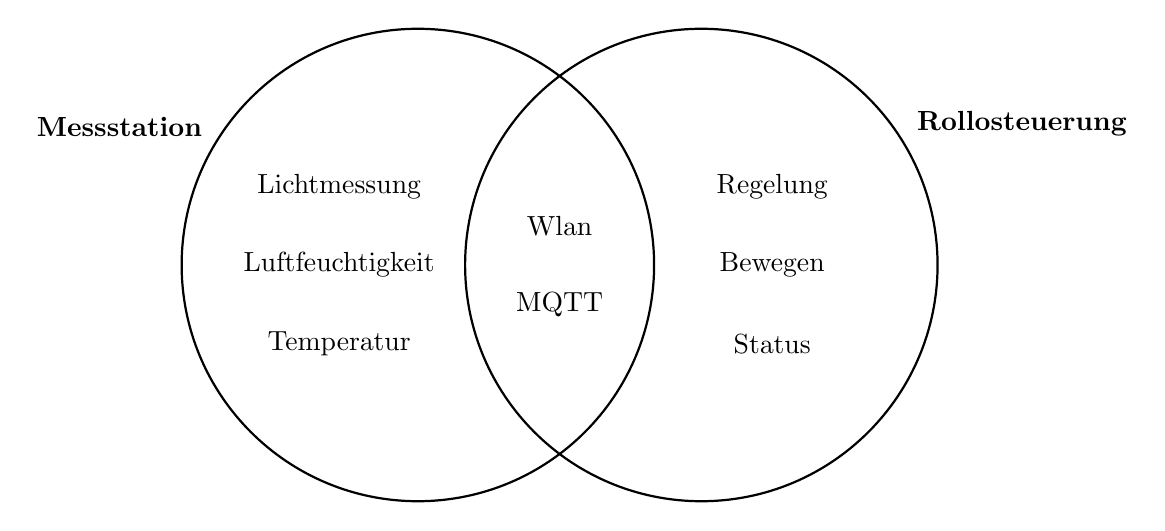
\begin{tikzpicture}[thick,
        set/.style = {circle,
            minimum size = 6cm,
        }]
     
        % Set A
        \node[set,label={150:\textbf{Messstation}}] (A) at (0,0) {};
        
        % Set B
        \node[set,label={30:\textbf{Rollosteuerung}}] (B) at (3.6,0) {};
        
        % Intersection
        \begin{scope}
            \clip (0,0) circle(3cm);
            \clip (3.6,0) circle(3cm);
        \end{scope}
        
        % Circles outline
        \draw (0,0) circle(3cm);
        \draw (3.6,0) circle(3cm);
        
        % Set intersection label
        \node at (1.8,0.5) {Wlan};
        \node at (1.8,-0.5) {MQTT};
        
        \node at (-1,1) {Lichtmessung};
        \node at (-1,0) {Luftfeuchtigkeit};
        \node at (-1,-1) {Temperatur};

        \node at (4.5,1) {Regelung};
        \node at (4.5,0) {Bewegen};
        \node at (4.5,-1) {Status};
     
    \end{tikzpicture}
    \caption{Darstellung der Verteilung von Funktionen der beiden Mikrocontroller}\label{fig:funk_schnitt}
\end{figure}

\section{Ablaufdiagramm}
\begin{figure}[H]
    \centering
    \begin{tikzpicture}[thick,scale=1, every node/.style={scale=1}]
        \node[activity] (callback){Nachricht};

        \node[decision,right = of callback] (decision1) {Funktion};

        \node[activity,above right  = 0.25cm  and 2cm   of decision1] (action1) {manuell()};
        \node[activity,above        = 0.7cm             of action1] (action2) {messung()};
        \node[activity,below right  = 0.25cm  and 2cm   of decision1] (action3) {automatik()};
        \node[activity,below        = 0.7cm             of action3] (action4) {Modus ändern};

        \node[end,below right       = 0.7cm   and 1cm   of action1](end){};

        \path [arrow line] (callback) -- (decision1);
        \path [arrow line] (decision1) |- node [above, near end]{steuerung}(action1);
        \path [arrow line] (decision1) |- node [above, near end]{status}(action2);
        \path [arrow line] (decision1) |- node [below, near end]{licht}(action3);
        \path [arrow line] (decision1) |- node [below, near end]{modus}(action4);

        \path [arrow line] (action1) -| (end);
        \path [arrow line] (action2) -| (end);
        \path [arrow line] (action3) -| (end);
        \path [arrow line] (action4) -| (end);
    \end{tikzpicture} 
    \caption{Ablaufdiagramm der Callback-Funktion}\label{fig:rollo_callback}
\end{figure}



